%%%%%%%%%%%%%%%%%%%%%%%%%%%%%%%%%%%%%%%%%
% Short Sectioned Assignment
% LaTeX Template
% Version 1.0 (5/5/12)
%
% This template has been downloaded from:
% http://www.LaTeXTemplates.com
%
% Original author:
% Frits Wenneker (http://www.howtotex.com)
%
% License:
% CC BY-NC-SA 3.0 (http://creativecommons.org/licenses/by-nc-sa/3.0/)
%
%%%%%%%%%%%%%%%%%%%%%%%%%%%%%%%%%%%%%%%%%

%----------------------------------------------------------------------------------------
%	PACKAGES AND OTHER DOCUMENT CONFIGURATIONS
%----------------------------------------------------------------------------------------

\documentclass[paper=a4, fontsize=11pt]{scrartcl} % A4 paper and 11pt font size

\usepackage[T1]{fontenc} % Use 8-bit encoding that has 256 glyphs
\usepackage{fourier} % Use the Adobe Utopia font for the document - comment this line to return to the LaTeX default
\usepackage[english]{babel} % English language/hyphenation
\usepackage{amsmath,amsfonts,amsthm} % Math packages
\usepackage[utf8]{inputenc}
\usepackage{graphicx}
\usepackage{tabularx}
\usepackage{longtable}
\usepackage{threeparttable}
\usepackage{booktabs}
\usepackage{listings}
\usepackage[numbered,autolinebreaks,useliterate]{mcode}
\usepackage{float}
\usepackage{algpseudocode}
\usepackage[tight,footnotesize]{subfigure}
\usepackage{cprotect}


\usepackage{lipsum} % Used for inserting dummy 'Lorem ipsum' text into the template

\usepackage{sectsty} % Allows customizing section commands
\allsectionsfont{\centering \normalfont\scshape} % Make all sections centered, the default font and small caps

\usepackage{fancyhdr} % Custom headers and footers
\pagestyle{fancyplain} % Makes all pages in the document conform to the custom headers and footers
\fancyhead{} % No page header - if you want one, create it in the same way as the footers below
\fancyfoot[L]{} % Empty left footer
\fancyfoot[C]{} % Empty center footer
\fancyfoot[R]{\thepage} % Page numbering for right footer
\renewcommand{\headrulewidth}{0pt} % Remove header underlines
\renewcommand{\footrulewidth}{0pt} % Remove footer underlines
\setlength{\headheight}{13.6pt} % Customize the height of the header

\numberwithin{equation}{section} % Number equations within sections (i.e. 1.1, 1.2, 2.1, 2.2 instead of 1, 2, 3, 4)
\numberwithin{figure}{section} % Number figures within sections (i.e. 1.1, 1.2, 2.1, 2.2 instead of 1, 2, 3, 4)
\numberwithin{table}{section} % Number tables within sections (i.e. 1.1, 1.2, 2.1, 2.2 instead of 1, 2, 3, 4)

\setlength\parindent{0pt} % Removes all indentation from paragraphs - comment this line for an assignment with lots of text

% new command for short vertical space
\newcommand{\vertbreak}{\vspace{1.75 mm}}

% define "struts", as suggested by Claudio Beccari in
%    a piece in TeX and TUG News, Vol. 2, 1993.
\newcommand\Tstrut{\rule{0pt}{2.6ex}}         % = `top' strut
\newcommand\Bstrut{\rule[-0.9ex]{0pt}{0pt}}   % = `bottom' strut

%----------------------------------------------------------------------------------------
%	TITLE SECTION
%----------------------------------------------------------------------------------------

\newcommand{\horrule}[1]{\rule{\linewidth}{#1}} % Create horizontal rule command with 1 argument of height

\title{	
\normalfont \normalsize 
\textsc{Faculdade de Engenharia da Universidade do Porto} \\ [25pt] % Your university, school and/or department name(s)
\horrule{0.5pt} \\[0.4cm] % Thin top horizontal rule
\LARGE Machnine Learning (PDEEC0049 : 15-782PP)\\ \Large Homework 4 \\ % The assignment title
\horrule{2pt} \\[0.5cm] % Thick bottom horizontal rule
}

\author{António Damião das Neves Rodrigues (200400437 : 700098386)} % Your name

\date{\normalsize\today} % Today's date or a custom date

\begin{document}

\maketitle % Print the title

\section{Problem 1}

\subsection{}
\label{subsec:1-1}

Starting from the dual representation for both $k_1(\textbf{x}_1;\textbf{x}_2)$ 
and $k_2(\textbf{x}_1;\textbf{x}_2) = 1 + k_1(\textbf{x}_1;\textbf{x}_2)$ we 
have expressions~\ref{eq:1-1-k1-dual-form} and~\ref{eq:1-1-k2-dual-form} 
respectively:

\begin{equation}
\begin{split}
    \arg\max_\lambda & \sum_{n=1}^{N}\lambda_n - \frac{1}{2}\sum_{n=1}^{N}\sum_{m=1}^{N}\lambda_n\lambda_{m}y_{n}y_{m}\lambda_nk_1(\textbf{x}_1;\textbf{x}_2)\\
    \\
    & \text{subject to}\\
    & 0 \le \lambda_n \le C\\
    & \sum_{n=1}^{N}\lambda_{n}y_{n} = 0
    \label{eq:1-1-k1-dual-form}
\end{split}
\end{equation}

\begin{equation}
\begin{split}
    \arg\max_\lambda & \sum_{n=1}^{N}\lambda_n - \frac{1}{2}\sum_{n=1}^{N}\sum_{m=1}^{N}\lambda_n\lambda_{m}y_{n}y_{m}\lambda_nk_2(\textbf{x}_1;\textbf{x}_2)\\
    \arg\max_\lambda & \sum_{n=1}^{N}\lambda_n - \frac{1}{2}\sum_{n=1}^{N}\sum_{m=1}^{N}\lambda_n\lambda_{m}y_{n}y_{m}\lambda_n(1 + k_1(\textbf{x}_1;\textbf{x}_2))\\
    \arg\max_\lambda & \sum_{n=1}^{N}\lambda_n - \frac{1}{2}\sum_{n=1}^{N}\sum_{m=1}^{N}\lambda_n\lambda_{m}y_{n}y_{m}\lambda_nk_1(\textbf{x}_1;\textbf{x}_2) - \frac{1}{2}\sum_{n=1}^{N}\sum_{m=1}^{N}\lambda_n\lambda_{m}y_{n}y_{m}\\
    \\
    & \text{subject to}\\
    & 0 \le \lambda_n \le C\\
    & \sum_{n=1}^{N}\lambda_{n}y_{n} = 0
    \label{eq:1-1-k2-dual-form}
\end{split}
\end{equation}

The quadratic programming optimization problems in 
expressions~\ref{eq:1-1-k2-dual-form} and~\ref{eq:1-1-k2-dual-form} differ on 
to the term $- \frac{1}{2}\sum_{n=1}^{N}\sum_{m=1}^{N}\lambda_n\lambda_{m}y_{n}y_{m}$. 
As one of the problem constraints is $\sum_{n=1}^{N}\lambda_{n}y_{n} = 0$, the 
term will be reduced to 0 during the solving process, and therefore the 
solutions will be essentially the same.

\subsection{}
\label{subsec:1-2}

\begin{equation*}
\begin{split}
    K(x,y) &= \phi_{\infty}(x).\phi_{\infty}(y) = \sum_{i=0}^{\infty}\frac{e^{-x^2/2}x^i}{\sqrt{i!}}\frac{e^{-y^2/2}y^i}{\sqrt{i!}}\\
    K(x,y) &= e^{-x^2/2}e^{-y^2/2}\sum_{i=0}^{\infty}\frac{x^iy^i}{i!}
    \label{eq:3-1-non-regular-normal}
\end{split}
\end{equation*}

where $\sum_{i=0}^{\infty}\frac{x^iy^i}{i!}$ is the Maclaurin series expansion for 
the exponential function~\cite{Abramowitz2012} $e^{xy}$, i.e. $\sum_{i=0}^{\infty}\frac{x^iy^i}{i!} = e^{xy}$. 
Therefore we have:

\begin{equation*}
\begin{split}
    K(x,y) &= e^{-x^2/2}e^{-y^2/2}\sum_{i=0}^{\infty}\frac{x^iy^i}{i!}\\
    K(x,y) &= e^{-x^2/2}e^{-y^2/2}e^{xy}\\
    K(x,y) &= e^{-x^2/2 - y^2/2 + xy}\\
    K(x,y) &= e^{\frac{-x^2 + 2xy - y^2}{2}}\\
    K(x,y) &= e^{\frac{-(x-y)^2}{2}}
    \label{eq:3-1-non-regular-normal}
\end{split}
\end{equation*}

\section{Problem 2}

Use the MATLAB code given as attachment (\verb+problem2+ folder) files 
\verb+basicSVM.m+ for implementation details. Follow the comments on the code 
for details and reasoning. The MATLAB file \verb+testSVM.m+ was used for 
testing the implementations.\vertbreak

Figures~\ref{fig:t-10-c-10} to~\ref{fig:t-100-c-10} compare the results obtained 
with the functions \verb+svmtrain()+ and \verb+svmpredict()+ of 
\verb+libsvm-mat-2.91-1+ and those obtained with the implemented 
\verb+basicSVM()+ for different values of training data size $T$ and a 
constraint value $C=10$.\vertbreak

\begin{figure}[H]
    \centering

    \subfigure[]{
        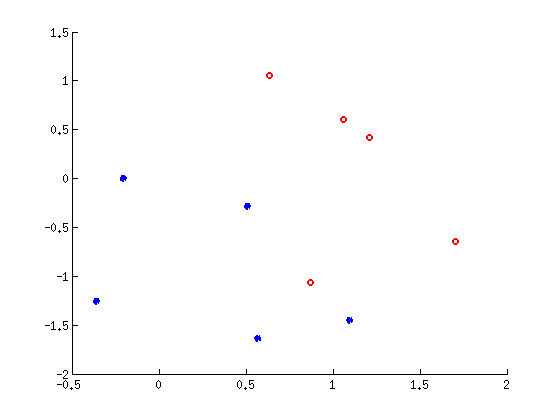
\includegraphics[width=0.50\textwidth] {figures/t-10-c-10-training.png}
        \label{subfig:t-10-c-10-training}
    }

    \subfigure[]{
        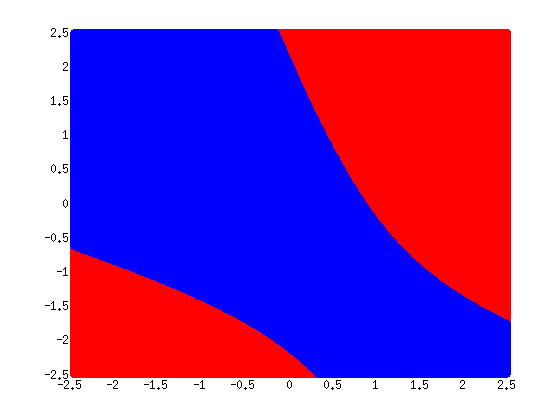
\includegraphics[width=0.50\textwidth] {figures/t-10-c-10-libsvm.png}
        \label{subfig:t-10-c-10-libsvm}
    }

    \subfigure[]{
        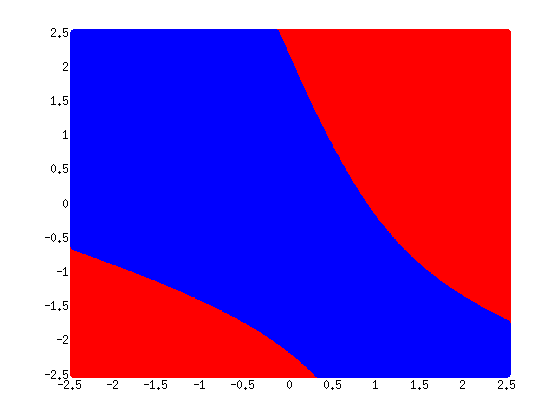
\includegraphics[width=0.50\textwidth] {figures/t-10-c-10-basicsvm.png}
        \label{subfig:t-10-c-10-basicsvm}
    }

    \cprotect\caption{Results of SVM classifiers, for $T = 10$ and $C = 10$: 
            training dataset (a),
            third-party \verb+libsvm-mat-2.91-1+ (b), \verb+basicSVM()+ (c).}
    \label{fig:t-10-c-10}

\end{figure}

\begin{figure}[H]
    \centering

    \subfigure[]{
        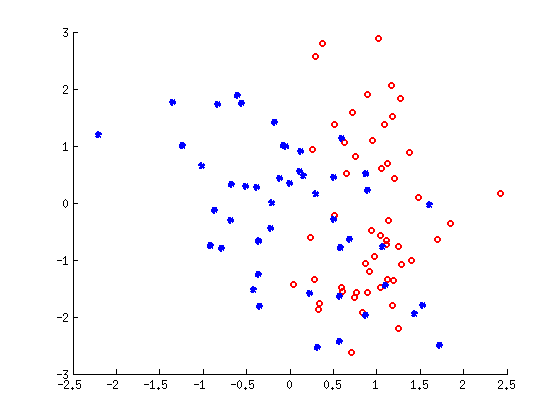
\includegraphics[width=0.50\textwidth] {figures/t-100-c-10-training.png}
        \label{subfig:t-100-c-10-training}
    }

    \subfigure[]{
        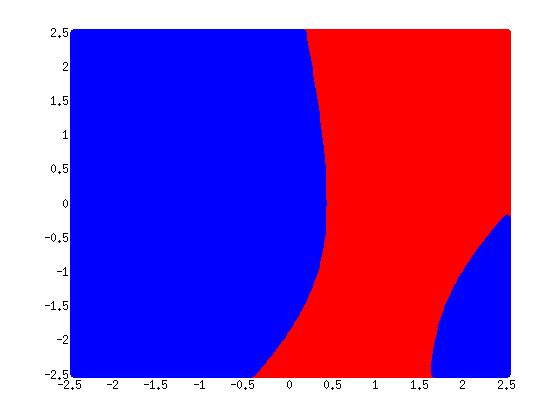
\includegraphics[width=0.50\textwidth] {figures/t-100-c-10-libsvm.png}
        \label{subfig:t-100-c-10-libsvm}
    }

    \subfigure[]{
        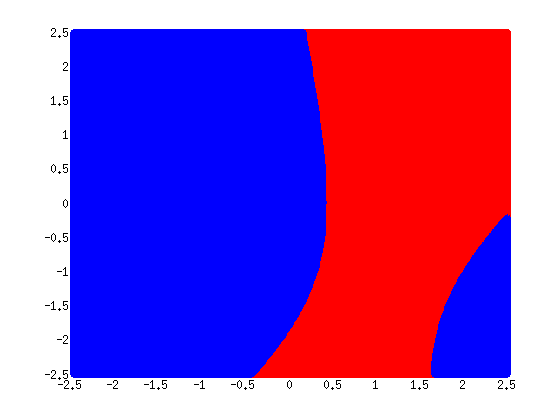
\includegraphics[width=0.50\textwidth] {figures/t-100-c-10-basicsvm.png}
        \label{subfig:t-100-c-10-basicsvm}
    }

    \cprotect\caption{Results of SVM classifiers, for $T = 100$ and $C = 10$: 
            training dataset (a),
            third-party \verb+libsvm-mat-2.91-1+ (b), \verb+basicSVM()+ (c).}
    \label{fig:t-100-c-10}

\end{figure}

\section{Problem 3}

Use the MATLAB code given as attachment (\verb+problem3+ folder), files 
\verb+SVM_DAG.m+, \verb+basicSVMtrain.m+ and \verb+basicSVMpredict.m+ for 
implementation details. Follow the comments on the code for details and 
reasoning. The MATLAB file \verb+testDAG.m+ was used for testing the 
implementations.\vertbreak

Figures~\ref{fig:t-500-c-1} to~\ref{fig:t-1000-c-1} compare the results obtained 
with the functions \verb+svmtrain()+ and \verb+svmpredict()+ of 
\verb+libsvm-mat-2.91-1+ and those obtained with the implemented 
\verb+basicSVM()+ for different values of training data size $T$ and 
$C=1$.\vertbreak

\begin{figure}[H]
    \centering

    \subfigure[]{
        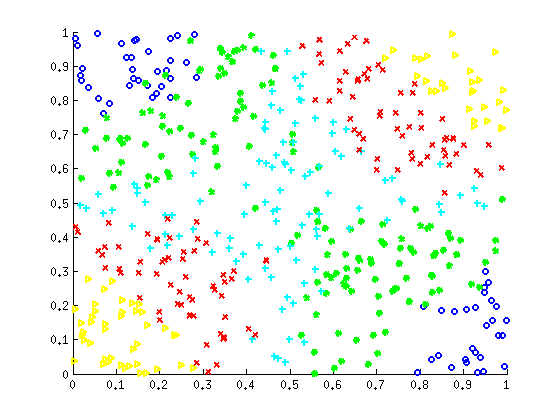
\includegraphics[width=0.50\textwidth] {figures/t-500-c-1-training.png}
        \label{subfig:t-500-c-1-training}
    }

    \subfigure[]{
        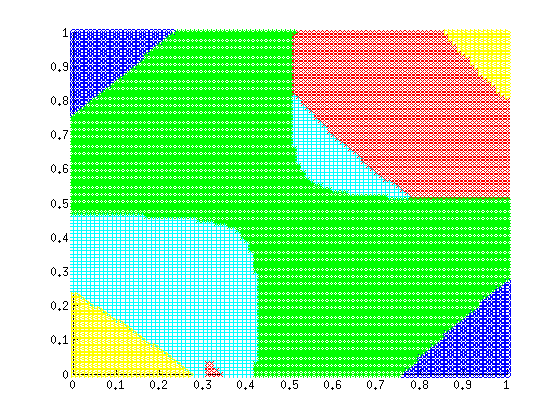
\includegraphics[width=0.50\textwidth] {figures/t-500-c-1-libsvm.png}
        \label{subfig:t-500-c-1-libsvm}
    }

    \subfigure[]{
        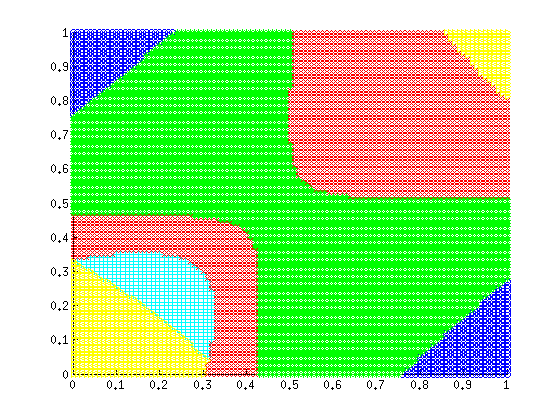
\includegraphics[width=0.50\textwidth] {figures/t-500-c-1-basicsvm.png}
        \label{subfig:t-500-c-1-basicsvm}
    }

    \cprotect\caption{Results of SVM classifiers, for $T = 500$ and $C = 1$: 
            training dataset (a),
            third-party \verb+libsvm-mat-2.91-1+ (b), \verb+basicSVM()+ (c).}
    \label{fig:t-500-c-1}

\end{figure}

\begin{figure}[H]
    \centering

    \subfigure[]{
        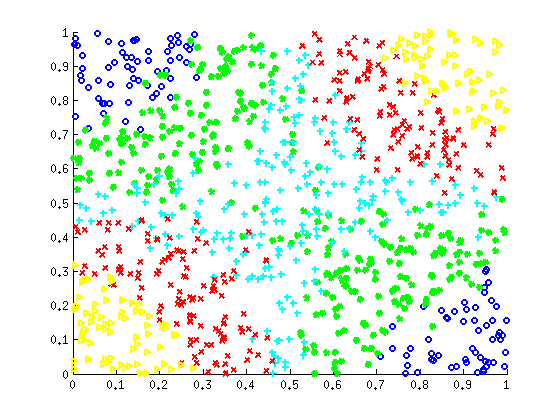
\includegraphics[width=0.50\textwidth] {figures/t-1000-c-1-training.png}
        \label{subfig:t-1000-c-1-training}
    }

    \subfigure[]{
        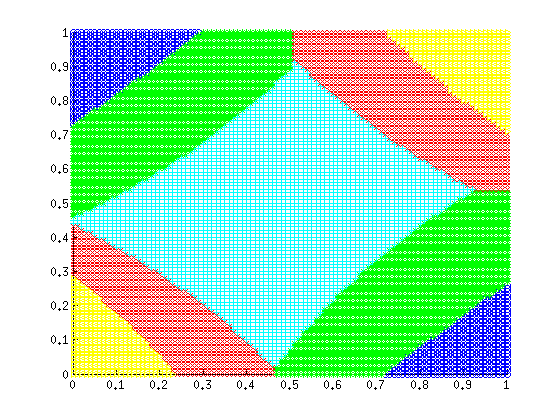
\includegraphics[width=0.50\textwidth] {figures/t-1000-c-1-libsvm.png}
        \label{subfig:t-1000-c-1-libsvm}
    }

    \subfigure[]{
        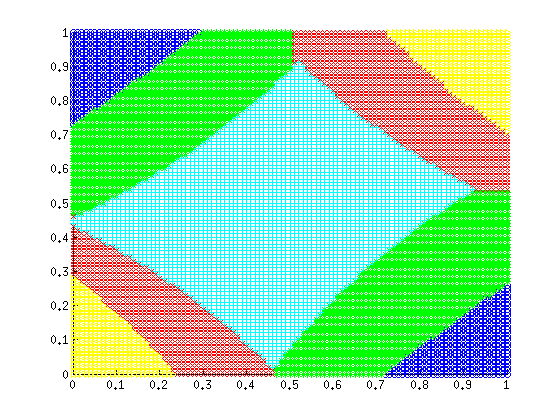
\includegraphics[width=0.50\textwidth] {figures/t-1000-c-1-basicsvm.png}
        \label{subfig:t-1000-c-1-basicsvm}
    }

    \cprotect\caption{Results of SVM classifiers, for $T = 1000$ and $C = 1$: 
            training dataset (a),
            third-party \verb+libsvm-mat-2.91-1+ (b), \verb+basicSVM()+ (c).}
    \label{fig:t-1000-c-1}

\end{figure}

\bibliographystyle{plain}
\bibliography{hw4.bib}

\end{document}
